%%%%%%%%%%%%%%%%%%%%%%%%%%%%%%%%%%%%%%%%%
% Simple Sectioned Essay Template
% LaTeX Template
%
% This template has been downloaded from:
% http://www.latextemplates.com
%
% Note:
% The \lipsum[#] commands throughout this template generate dummy text
% to fill the template out. These commands should all be removed when 
% writing essay content.
%
%%%%%%%%%%%%%%%%%%%%%%%%%%%%%%%%%%%%%%%%%

%----------------------------------------------------------------------------------------
%	PACKAGES AND OTHER DOCUMENT CONFIGURATIONS
%----------------------------------------------------------------------------------------

\documentclass[12pt]{article} % Default font size is 12pt, it can be changed here

\usepackage{geometry} % Required to change the page size to A4
\geometry{a4paper} % Set the page size to be A4 as opposed to the default US Letter

\usepackage{graphicx} % Required for including pictures

\usepackage{float} % Allows putting an [H] in \begin{figure} to specify the exact location of the figure
\usepackage{wrapfig} % Allows in-line images such as the example fish picture

\usepackage{lipsum} % Used for inserting dummy 'Lorem ipsum' text into the template

\linespread{1.2} % Line spacing

%\setlength\parindent{0pt} % Uncomment to remove all indentation from paragraphs

\graphicspath{{images/}} % Specifies the directory where pictures are stored

\begin{document}

%----------------------------------------------------------------------------------------
%	TITLE PAGE
%----------------------------------------------------------------------------------------

\begin{titlepage}

\newcommand{\HRule}{\rule{\linewidth}{0.5mm}} % Defines a new command for the horizontal lines, change thickness here

\center % Center everything on the page

\HRule \\[0.4cm]
{ \huge \bfseries Gifs and Musics}\\[0.4cm] % Title of your document
\HRule \\[1.5cm]

%\begin{minipage}{0.4\textwidth}
%\begin{flushleft} \large
\emph{Author:}\\
Daniel \textsc{Cravi\'ee} % Your name
\HRule \\[1.5cm]

%\end{flushleft}
%\end{minipage}
%~
%\begin{minipage}{0.4\textwidth}
%\begin{flushright} \large
%%\emph{Supervisor:} \\
%Dr. James \textsc{Smith} % Supervisor's Name
%\end{flushright}
%\end{minipage}\\[4cm]

{\large \today}\\[3cm] % Date, change the \today to a set date if you want to be precise

%\includegraphics{Logo}\\[1cm] % Include a department/university logo - this will require the graphicx package

\vfill % Fill the rest of the page with whitespace

\end{titlepage}

%----------------------------------------------------------------------------------------
%	TABLE OF CONTENTS
%----------------------------------------------------------------------------------------

\tableofcontents % Include a table of contents

\newpage % Begins the essay on a new page instead of on the same page as the table of contents 

%----------------------------------------------------------------------------------------
%	INTRODUCTION
%----------------------------------------------------------------------------------------


\section{Introduction} % Major section

This work explains the motive, the tecnology behind and of course, what is the \textit{Gifs and Musics} program.

The program is basically a web page that has many slides. Each one of this slides has a gif background and a music.
 
You could also ask me why this essay is so short, and that is because there is no much to say.

The code of this project can be found in my Github \cite{craviee}, and the published version of this work can be found in Heroku \cite{heroku}.
	

%------------------------------------------------

\subsection{Motive} % Sub-section

This is a good question, the reason why I made this program is that I thought it was a good idea, no more and no less.

Sorry, I can not control myself.

%------------------------------------------------

\subsection{Tecnology} % Sub-section
\label{sec:tec}

Well, since this program is a web page, we have HTML, CSS and JS.
It is important to say that the music that plays in the page is from youtube.

%------------------------------------------------


%----------------------------------------------------------------------------------------
%	DEVELOPMENT
%----------------------------------------------------------------------------------------

\section{Development} % Major section

As I said in Section \ref{sec:tec} in this work we have HTML, CSS and JS.

The function of HTML is place the elements that the JS will change, and the CSS will stylize. This is the case of the Youtube box and buttons. The function of CSS is to stylize the page, and apply some cool effects, like round corners and place the wallpaper. The function of JS is to change elements of JS. When I press a button to move to the next slide, the JS will change the background and play another music of Youtube.

It is a very simple program.

%------------------------------------------------

\subsection{Images} % Sub-section

\begin{figure}[h]
\centering
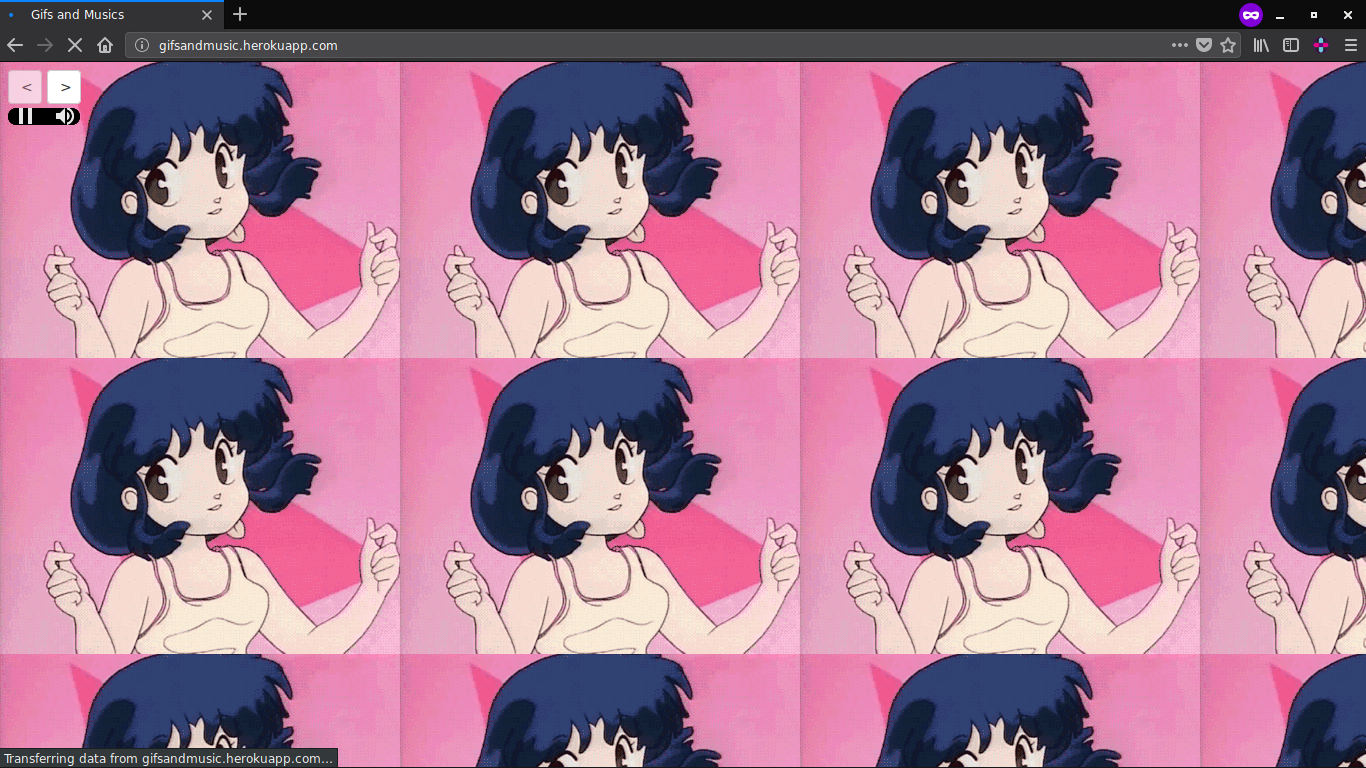
\includegraphics[scale=.37]{1.png}
\caption{This is the first gif you will see in the website.}
\label{figure1}
\end{figure}

Besides the wallpaper, in Figure \ref{figure1} you can see in the north-west region two buttons and one black box.

The function of those buttons is to change to the next pair of gif and music. The reason why de left button is disabled is because this is the first pair, in other words, there is no pair behind the first one.

The function of the black box is to play a Youtube song, where you can pause and mute the music.

\begin{figure}[h]
\centering

\includegraphics[scale=.37]{2.png}
\caption{Another pair of gif and music.}
\label{figure2}
\end{figure}

In Figure \ref{figure2} you can see that the first button isn't disabled anymore, that can be explained because there is a pair behind this current pair.

\begin{figure}[H]
\centering

\includegraphics[scale=.37]{3.png}
\caption{Example of last pair of gif and music.}
\label{figure3}
\end{figure}

The reason why the right button is disabled in Figure \ref{figure3} is obvious, it is because this is the current last pair of gif and music.

\subsection{Run}

You have two options to run this program.

\subsubsection{Online}
The first one is the simplest and basically you just need to access the published website \cite{heroku}.

\subsubsection{Local}
Or you can follow these steps of cloning my Github repo \cite{craviee}
\begin{enumerate}

	\item Open a Linux terminal
	
	\item Type: git clone https://github.com/craviee/GifsAndMusic.git
	
	\item Go to the folder you just downloaded and go to html folder
	
	\item Open the home.html with your favourite browser
	
\end{enumerate}

%----------------------------------------------------------------------------------------
%	MAJOR SECTION X - TEMPLATE - UNCOMMENT AND FILL IN
%----------------------------------------------------------------------------------------

%\section{Content Section}

%\subsection{Subsection 1} % Sub-section

% Content

%------------------------------------------------

%\subsection{Subsection 2} % Sub-section

% Content

%----------------------------------------------------------------------------------------
%	CONCLUSION
%----------------------------------------------------------------------------------------

\section{Conclusion} % Major section

Don't use drugs, kids.

%----------------------------------------------------------------------------------------
%	BIBLIOGRAPHY
%----------------------------------------------------------------------------------------

\begin{thebibliography}{99} % Bibliography - this is intentionally simple in this template

\bibitem[Cravi\'ee, 2018]{craviee}
https://github.com/craviee/GifsAndMusic

\bibitem[Gifs And Music, 2018]{heroku}
http://gifsandmusic.herokuapp.com/
 
\end{thebibliography}

%----------------------------------------------------------------------------------------

\end{document}